\onecolumn
\section{Derivation of Meta-Multiagent Policy Gradient Theorem}\label{sec:proof-meta-multiagent-pg}
\textbf{Theorem 1.} (Meta-Multiagent Policy Gradient Theorem) \textit{For any stochastic game $\mathcal{M}_{n}$, the gradient of the meta-value function for agent $i$ at state $s_0$ with respect to current policy parameters $\phi_0^i$ evolving in the environment along with other peer agents using initial parameters $\bm{\phi}_{\bm{0}}^{\bm{-i}}$ is:}
\begin{align*}
\begin{split}
&\nabla_{\phi^{i}_{0}}V^{i}_{\bm{\phi}_{\bm{0:\ell+1}}}(s_0,\phi^{i}_{0})=\mathbb{E}_{p(\tau_{\bm{\phi}_{\bm{0:\ell}}}|\bm{\phi}_{\bm{0:\ell}})}\Big[\mathbb{E}_{p(\tau_{\bm{\phi}_{\bm{\ell+1}}}|\bm{\phi}_{\bm{\ell+1}})}\big[G^{i}(\tau_{\bm{\phi}_{\bm{\ell+1}}})\\
&\;\;\big(\underbrace{\nabla_{\phi^{i}_{0}}\log\pi(\tau_{\bm{\phi}_{\bm{0}}}|\phi^{i}_{0})}_{\text{Current Policy}}+\underbrace{\smallsum\nolimits_{\ell'=0}^{\ell}\nabla_{\phi^{i}_{0}}\log\pi(\tau_{\bm{\phi}_{\bm{\ell'+1}}}|\phi^{i}_{\ell'+1})}_{\text{Own Learning}}+\underbrace{\smallsum\nolimits_{\ell'=0}^{\ell}\nabla_{\phi^{i}_{0}}\log\pi(\tau_{\bm{\phi}_{\bm{\ell'+1}}}|\bm{\phi}^{\bm{-i}}_{\bm{\ell'+1}})}_{\text{Peer Learning}}\big)\big]\Big].
\end{split}
\end{align*}
\begin{proof}
We begin our derivation from the meta-value function defined in~\Cref{eqn:meta-value-function} and expand it with the state-action value and joint actions, assuming the conditional independence between agents' actions~\citep{wen2018probabilistic}: 
\begin{align}\label{eqn:theorem-step1}
\begin{split}
V^{i}_{\bm{\phi}_{\bm{0:\ell+1}}}(s_0,\phi^{i}_{0})=
&\mathbb{E}_{{p(\tau_{\bm{\phi}_{\bm{0:\ell}}}}|\bm{\phi}_{\bm{0:\ell}})}\Big[\mathbb{E}_{\tau_{\bm{\phi}_{\bm{\ell+1}}}}\big[G^{i}(\tau_{\bm{\phi}_{\bm{\ell+1}}})\big]\Big]=\mathbb{E}_{{p(\tau_{\bm{\phi}_{\bm{0:\ell}}}}|\bm{\phi}_{\bm{0:\ell}})}\Big[V^{i}_{\bm{\phi}_{\bm{\ell+1}}}(s_0)\Big]\\
=&\mathbb{E}_{{p(\tau_{\bm{\phi}_{\bm{0:\ell}}}}|\bm{\phi}_{\bm{0:\ell}})}\Big[\smallsum_{a^{i}_{0}}\pi(a^{i}_{0}|s_0,\phi^{i}_{\ell+1})\smallsum_{\bm{a}^{\bm{-i}}_{\bm{0}}}\bm{\pi}(\bm{a}^{\bm{-i}}_{\bm{0}}|s_{0},\bm{\phi}^{\bm{-i}}_{\bm{\ell+1}}) Q^{i}_{\bm{\phi}_{\bm{\ell+1}}}(s_{0},\bm{a}_{\bm{0}})\Big],
\end{split}
\end{align}
where $Q^{i}_{\bm{\phi}_{\bm{\ell+1}}}(s_{0},\bm{a}_{\bm{0}})$ is the state-action value under the joint policy with parameters $\bm{\phi}_{\bm{\ell+1}}$ at state $s_{0}$ with joint action $\bm{a}_{\bm{0}}$.

In~\cref{eqn:theorem-step1}, we note that both $\bm{\phi}^{\bm{i}}_{\bm{1:\ell}}$ and $\bm{\phi}^{\bm{-i}}_{\bm{1:\ell}}$ depend on $\phi^{i}_{0}$. 
Considering the joint update from $\bm{\phi}_{\bm{0}}$ to $\bm{\phi}_{\bm{1}}$, for simplicity, we can write the gradients in the inner-loop (see \Cref{eqn:inner-loop}) based on the multiagent stochastic policy gradient theorem~\citep{wei18multiagent-softQ}:
\begin{align}\label{eqn:theorem-step2}
\begin{split}
\nabla_{\phi^{-i}_{0}}\mathbb{E}_{p(\tau_{\bm{\phi}_{\bm{0}}}|\bm{\phi}_{\bm{0}})}\Big[G^{i}(\tau_{\bm{\phi}_{\bm{0}}})\Big]&=\smallsum_{s}\rho_{\bm{\phi}_{\bm{0}}}(s)\smallsum_{a^{i}}\nabla_{\phi^{i}_{0}}\pi(a^{i}|s,\phi^{i}_{0})\smallsum_{\bm{a}^{\bm{-i}}}\bm{\pi}(\bm{a}^{\bm{-i}}|s,\bm{\phi}^{\bm{-i}}_{\bm{0}})Q^{i}_{\bm{\phi}_{\bm{0}}}(s,\bm{a}),\\
\nabla_{\bm{\phi}^{\bm{-i}}_{\bm{0}}}\mathbb{E}_{p(\tau_{\bm{\phi}_{\bm{0}}}|\bm{\phi}_{\bm{0}})}\Big[\bm{G}^{\bm{-i}}(\tau_{\bm{\phi}_{\bm{0}}})\Big]&=\smallsum_{s}\rho_{\bm{\phi}_{\bm{0}}}(s)\smallsum_{\bm{a}^{\bm{-i}}}\nabla_{\bm{\phi}^{\bm{-i}}_{\bm{0}}}\bm{\pi}(\bm{a}^{\bm{-i}}|s,\bm{\phi}^{\bm{-i}}_{\bm{0}})\smallsum_{a^{i}}\pi(a^{i}|s,\phi^{i}_{0})\bm{Q}^{\bm{-i}}_{\bm{\phi}_{\bm{0}}}(s,\bm{a}),
\end{split}
\end{align}
where $\rho_{\bm{\phi}_{\bm{0}}}$ denotes the stationary distribution under the joint policy with parameters $\bm{\phi}_{\bm{0}}$.
Importantly, the inner-loop gradients for an agent $i$ and its peers are a function of $\phi^{i}_{0}$. 
Hence, the updated joint policy parameter $\bm{\phi}_{\bm{1}}$ depends on $\phi^{i}_{0}$. 
Following~\Cref{eqn:theorem-step2}, the successive inner-loop optimization until $\bm{\phi}_{\bm{\ell+1}}$ results in dependencies between $\phi^{i}_{0}$ and $\bm{\phi}^{\bm{i}}_{\bm{1:\ell+1}}$ and between $\phi^{i}_{0}$ and $\bm{\phi}^{\bm{-i}}_{\bm{1:\ell+1}}$ (see~\cref{fig:graph-meta-mapg}).

Having identified which terms are dependent on $\phi^{i}_{0}$, we continue from~\cref{eqn:theorem-step1} and derive the gradient of the meta-value function with respect to $\phi^{i}_{0}$ by applying the product rule:
\begin{align}\label{eqn:theorem-step3}
\nabla_{\phi^{i}_{0}}V^{i}_{\bm{\phi}_{\bm{0:\ell+1}}}(s_0,\phi^{i}_{0})&=\nabla_{\phi^{i}_{0}}\Big[\mathbb{E}_{{p(\tau_{\bm{\phi}_{\bm{0:\ell}}}}|\bm{\phi}_{\bm{0:\ell}})}\Big[\smallsum_{a^{i}_{0}}\pi(a^{i}_{0}|s_0,\phi^{i}_{\ell+1})\smallsum_{\bm{a}^{\bm{-i}}_{\bm{0}}}\bm{\pi}(\bm{a}^{\bm{-i}}_{\bm{0}}|s_{0},\bm{\phi}^{\bm{-i}}_{\bm{\ell+1}}) Q^{i}_{\bm{\phi}_{\bm{\ell+1}}}(s_{0},\bm{a}_{\bm{0}})\Big]\Big]\nonumber\\
&=\nabla_{\phi^{i}_{0}}\Big[\smallsum_{\tau_{\bm{\phi}_{\bm{0:\ell}}}} p(\tau_{\bm{\phi}_{\bm{0:\ell}}}|\bm{\phi}^{\bm{i}}_{\bm{0:\ell}},\bm{\phi}^{\bm{-i}}_{\bm{0:\ell}})\smallsum_{a^{i}_{0}}\pi(a^{i}_{0}|s_0,\phi^{i}_{\ell+1})\smallsum_{\bm{a}^{\bm{-i}}_{\bm{0}}}\bm{\pi}(\bm{a}^{\bm{-i}}_{\bm{0}}|s_{0},\bm{\phi}^{\bm{-i}}_{\bm{\ell+1}}) Q^{i}_{\bm{\phi}_{\bm{\ell+1}}}(s_{0},\bm{a}_{\bm{0}})\Big]\nonumber\\
&=\underbrace{\nabla_{\phi^{i}_{0}}\Big[\smallsum_{\tau_{\bm{\phi}_{\bm{0:\ell}}}} p(\tau_{\bm{\phi}_{\bm{0:\ell}}}|\bm{\phi}^{\bm{i}}_{\bm{0:\ell}},\bm{\phi}^{\bm{-i}}_{\bm{0:\ell}})\Big]\smallsum_{a^{i}_{0}}\pi(a^{i}_{0}|s_0,\phi^{i}_{\ell+1})\smallsum_{\bm{a}^{\bm{-i}}_{\bm{0}}}\bm{\pi}(\bm{a}^{\bm{-i}}_{\bm{0}}|s_{0},\bm{\phi}^{\bm{-i}}_{\bm{\ell+1}}) Q^{i}_{\bm{\phi}_{\bm{\ell+1}}}(s_{0},\bm{a}_{\bm{0}})}_{\text{Term A}}+\nonumber\\
&\;\;\;\;\:\underbrace{\smallsum_{\tau_{\bm{\phi}_{\bm{0:\ell}}}} p(\tau_{\bm{\phi}_{\bm{0:\ell}}}|\bm{\phi}^{\bm{i}}_{\bm{0:\ell}},\bm{\phi}^{\bm{-i}}_{\bm{0:\ell}})\Big[\smallsum_{a^{i}_{0}}\nabla_{\phi^{i}_{0}}\pi(a^{i}_{0}|s_0,\phi^{i}_{\ell+1})\Big]\smallsum_{\bm{a}^{\bm{-i}}_{\bm{0}}}\bm{\pi}(\bm{a}^{\bm{-i}}_{\bm{0}}|s_{0},\bm{\phi}^{\bm{-i}}_{\bm{\ell+1}}) Q^{i}_{\bm{\phi}_{\bm{\ell+1}}}(s_{0},\bm{a}_{\bm{0}})}_{\text{Term B}}+\\
&\;\;\;\;\:\underbrace{\smallsum_{\tau_{\bm{\phi}_{\bm{0:\ell}}}} p(\tau_{\bm{\phi}_{\bm{0:\ell}}}|\bm{\phi}^{\bm{i}}_{\bm{0:\ell}},\bm{\phi}^{\bm{-i}}_{\bm{0:\ell}})\smallsum_{a^{i}_{0}}\pi(a^{i}_{0}|s_0,\phi^{i}_{\ell+1})\Big[\smallsum_{\bm{a}^{\bm{-i}}_{\bm{0}}}\nabla_{\phi^{i}_{0}}\bm{\pi}(\bm{a}^{\bm{-i}}_{\bm{0}}|s_{0},\bm{\phi}^{\bm{-i}}_{\bm{\ell+1}})\Big] Q^{i}_{\bm{\phi}_{\bm{\ell+1}}}(s_{0},\bm{a}_{\bm{0}})}_{\text{Term C}}+\nonumber\\
&\;\;\;\;\:\underbrace{\smallsum_{\tau_{\bm{\phi}_{\bm{0:\ell}}}} p(\tau_{\bm{\phi}_{\bm{0:\ell}}}|\bm{\phi}^{\bm{i}}_{\bm{0:\ell}},\bm{\phi}^{\bm{-i}}_{\bm{0:\ell}})\smallsum_{a^{i}_{0}}\pi(a^{i}_{0}|s_0,\phi^{i}_{\ell+1})\smallsum_{\bm{a}^{\bm{-i}}_{\bm{0}}}\bm{\pi}(\bm{a}^{\bm{-i}}_{\bm{0}}|s_{0},\bm{\phi}^{\bm{-i}}_{\bm{\ell+1}})\Big[\nabla_{\phi^{i}_{0}}Q^{i}_{\bm{\phi}_{\bm{\ell+1}}}(s_{0},\bm{a}_{\bm{0}})\Big]}_{\text{Term D}}\nonumber.
\end{align}
We first focus on the derivative of the trajectories $\tau_{\bm{\phi}_{\bm{0:\ell}}}$ in Term A:
\begin{align}\label{eqn:theorem-step4}
\begin{split}
\nabla_{\phi^{i}_{0}}\Big[\smallsum_{\tau_{\bm{\phi}_{\bm{0:\ell}}}} p(\tau_{\bm{\phi}_{\bm{0:\ell}}}|\bm{\phi}^{\bm{i}}_{\bm{0:\ell}},\bm{\phi}^{\bm{-i}}_{\bm{0:\ell}})\Big]&=\nabla_{\phi^{i}_{0}}\Big[\smallsum_{\tau_{\bm{\phi}_{\bm{0}}}} p(\tau_{\bm{\phi}_{\bm{0}}}|\phi^{i}_{0},\bm{\phi}^{\bm{-i}}_{\bm{0}})\smallsum_{\tau_{\bm{\phi}_{\bm{1}}}} p(\tau_{\bm{\phi}_{\bm{1}}}|\phi^{i}_{1},\bm{\phi}^{\bm{-i}}_{\bm{1}})\times\sdots\times\smallsum_{\tau_{\bm{\phi}_{\bm{\ell}}}} p(\tau_{\bm{\phi}_{\bm{\ell}}}|\phi^{i}_{\ell},\bm{\phi}^{\bm{-i}}_{\bm{\ell}})\Big]\\
&=\Big[\smallsum_{\tau_{\bm{\phi}_{\bm{0}}}}\nabla_{\phi^{i}_{0}} p(\tau_{\bm{\phi}_{\bm{0}}}|\phi^{i}_{0},\bm{\phi}^{\bm{-i}}_{\bm{0}})\Big]\textstyle\prod_{\forall\ell'\in\{0,\sdots,\ell\}\setminus \{0\}}\smallsum_{\tau_{\bm{\phi}_{\bm{\ell'}}}} p(\tau_{\bm{\phi}_{\bm{\ell'}}}|\phi^{i}_{\ell'},\bm{\phi}^{\bm{-i}}_{\bm{\ell'}})+\\
&\;\;\;\;\:\Big[\smallsum_{\tau_{\bm{\phi}_{\bm{1}}}}\nabla_{\phi^{i}_{1}} p(\tau_{\bm{\phi}_{\bm{1}}}|\phi^{i}_{1},\bm{\phi}^{\bm{-i}}_{\bm{1}})\Big]\textstyle\prod_{\forall\ell'\in\{0,\sdots,\ell\}\setminus \{1\}}\smallsum_{\tau_{\bm{\phi}_{\bm{\ell'}}}} p(\tau_{\bm{\phi}_{\bm{\ell'}}}|\phi^{i}_{\ell'},\bm{\phi}^{\bm{-i}}_{\bm{\ell'}})+\sdots+\\
&\;\;\;\;\:\Big[\smallsum_{\tau_{\bm{\phi}_{\bm{\ell}}}}\nabla_{\phi^{i}_{\ell}} p(\tau_{\bm{\phi}_{\bm{\ell}}}|\phi^{i}_{\ell},\bm{\phi}^{\bm{-i}}_{\bm{\ell}})\Big]\textstyle\prod_{\forall\ell'\in\{0,\sdots,\ell\}\setminus \{\ell\}}\smallsum_{\tau_{\bm{\phi}_{\bm{\ell'}}}} p(\tau_{\bm{\phi}_{\bm{\ell'}}}|\phi^{i}_{\ell'},\bm{\phi}^{\bm{-i}}_{\bm{\ell'}}),
\end{split}
\end{align}
where the probability of collecting a trajectory under the joint policy with parameters $\bm{\phi}_{\bm{\ell}}$ is given by:
\begin{align}\label{eqn:theorem-step5}
\begin{split}
p(\tau_{\bm{\phi}_{\bm{\ell}}}|\phi^{i}_{\ell},\bm{\phi}^{\bm{-i}}_{\bm{\ell}})=p(s_0)\textstyle\prod\nolimits_{t=0}^{H}\pi(a^{i}_{t}|s_{t},\phi^{i}_{\ell})\bm{\pi}(\bm{a}^{\bm{-i}}_{\bm{t}}|s_{t},\bm{\phi}^{\bm{-i}}_{\bm{\ell}})\mathcal{P}(s_{t+1}|s_{t},\bm{a}_{\bm{t}}).
\end{split}
\end{align}

Using~\cref{eqn:theorem-step5} and the log-derivative trick,~\cref{eqn:theorem-step4} can be further expressed as:
\begin{align}\label{eqn:theorem-step6}
\begin{split}
&\Big[\mathbb{E}_{p(\tau_{\bm{\phi}_{\bm{0}}}|\bm{\phi}_{\bm{0}})}\nabla_{\phi^{i}_{0}}\log\pi(\tau_{\bm{\phi}_{\bm{0}}}|\phi^{i}_{0})\Big]\textstyle\prod\nolimits_{\forall\ell'\in\{0,\sdots,\ell\}\setminus \{0\}}\smallsum_{\tau_{\bm{\phi}_{\bm{\ell'}}}}p(\tau_{\bm{\phi}_{\bm{\ell'}}}|\phi^{i}_{\ell'},\bm{\phi}^{\bm{-i}}_{\bm{\ell'}})+\\
&\Big[\mathbb{E}_{p(\tau_{\bm{\phi}_{\bm{1}}}|\bm{\phi}_{\bm{1}})}\nabla_{\phi^{i}_{0}}\Big(\log\pi(\tau_{\bm{\phi}_{\bm{1}}}|\phi^{i}_{1})+\log\bm{\pi}(\tau_{\bm{\phi}_{\bm{1}}}|\bm{\phi}^{\bm{-i}}_{\bm{1}})\Big)\Big]\textstyle\prod\nolimits_{\forall\ell'\in\{0,\sdots,\ell\}\setminus \{1\}}\smallsum_{\tau_{\bm{\phi}_{\bm{\ell'}}}}p(\tau_{\bm{\phi}_{\bm{\ell'}}}|\phi^{i}_{\ell'},\bm{\phi}^{\bm{-i}}_{\bm{\ell'}})+\sdots+\\
&\Big[\mathbb{E}_{p(\tau_{\bm{\phi}_{\bm{\ell}}}|\bm{\phi}_{\bm{\ell}})}\nabla_{\phi^{i}_{0}}\Big(\log\pi(\tau_{\bm{\phi}_{\bm{\ell}}}|\phi^{i}_{\ell})+\log\bm{\pi}(\tau_{\bm{\phi}_{\bm{\ell}}}|\bm{\phi}^{\bm{-i}}_{\bm{\ell}})\Big)\Big]\textstyle\prod\nolimits_{\forall\ell'\in\{0,\sdots,\ell\}\setminus \{\ell\}}\smallsum_{\tau_{\bm{\phi}_{\bm{\ell'}}}}p(\tau_{\bm{\phi}_{\bm{\ell'}}}|\phi^{i}_{\ell'},\bm{\phi}^{\bm{-i}}_{\bm{\ell'}})
\end{split}
\end{align}
where the summations of the log-terms, such as $\nabla_{\phi^{i}_{0}}\!\Big(\!\log\pi(\tau_{\bm{\phi}_{\bm{\ell}}}|\phi^{i}_{\ell})\!+\!\log\bm{\pi}(\tau_{\bm{\phi}_{\bm{\ell}}}|\bm{\phi}^{\bm{-i}}_{\bm{\ell}})\!\Big)$ are \textit{inherently} included due to the sequential dependencies between $\phi^{i}_{0}$ and $\bm{\phi}_{\bm{1:\ell}}$. We use the result of~\cref{eqn:theorem-step6} and organize terms to arrive at the following expression for Term A in~\Cref{eqn:theorem-step3}:
\begin{align}\label{eqn:theorem-step7}
\begin{split}
\mathbb{E}_{p(\tau_{\bm{\phi}_{\bm{0:\ell}}}|\bm{\phi}_{\bm{0:\ell}})}\Big[&\Big(\nabla_{\phi^{i}_{0}}\log\pi(\tau_{\bm{\phi}_{\bm{0}}}|\phi^{i}_{0})+\smallsum_{\ell'=0}^{\ell-1}\nabla_{\phi^{i}_{0}}\log\pi(\tau_{\bm{\phi_{\ell'+1}}}|\phi^{i}_{\ell'+1})+\smallsum_{\ell'=0}^{\ell-1}\nabla_{\phi^{i}_{0}}\log\pi(\tau_{\bm{\phi_{\ell'+1}}}|\bm{\phi}^{\bm{-i}}_{\bm{\ell'+1}})\Big)\times\\
&\;\smallsum_{a^{i}_{0}}\pi(a^{i}_{0}|s_0,\phi^{i}_{\ell+1})\smallsum_{\bm{a}^{\bm{-i}}_{\bm{0}}}\bm{\pi}(\bm{a}^{\bm{-i}}_{\bm{0}}|s_{0},\bm{\phi}^{\bm{-i}}_{\bm{\ell+1}}) Q^{i}_{\bm{\phi}_{\bm{\ell+1}}}(s_{0},\bm{a}_{\bm{0}})
\Big].
\end{split}
\end{align}
Coming back to Term B-D in~\Cref{eqn:theorem-step3}, repeatedly unrolling the derivative of the Q-function $\nabla_{\phi^{i}_{0}}Q^{i}_{\bm{\phi}_{\bm{\ell+1}}}(s_{0},\bm{a}_{\bm{0}})$ by following~\citet{Sutton:1998} yields:
\begin{align}\label{eqn:theorem-step8}
\begin{split}
&
\mathbb{E}_{{p(\tau_{\bm{\phi}_{\bm{0:\ell}}}}|\bm{\phi}_{\bm{0:\ell}})}\Big[\smallsum_{s}\rho_{\bm{\phi}_{\bm{\ell+1}}}(s)\smallsum_{a^{i}}\nabla_{\phi^{i}_{0}}\pi(a^{i}|s,\phi^{i}_{\ell+1})\smallsum_{\bm{a}^{\bm{-i}}}\bm{\pi}(\bm{a}^{\bm{-i}}|s,\bm{\phi}^{\bm{-i}}_{\bm{\ell+1}})Q^{i}_{\bm{\phi}+1}(s,\bm{a})\Big]+\\
&
\mathbb{E}_{{p(\tau_{\bm{\phi}_{\bm{0:\ell}}}|\bm{\phi}_{\bm{0:\ell}})}}
\Big[\smallsum_{s}\rho_{\bm{\phi}_{\bm{\ell+1}}}(s)\smallsum_{\bm{a}^{\bm{-i}}}\nabla_{\phi^{i}_{0}}\bm{\pi}(\bm{a}^{\bm{-i}}|s,\bm{\phi}^{\bm{-i}}_{\bm{\ell+1}})\smallsum_{a^{i}}\pi(a^{i}|s,\phi^{i}_{\ell+1})Q^{i}_{\bm{\phi}_{\bm{\ell+1}}}(s,\bm{a})\Big],
\end{split}
\end{align}
which adds the consideration of future joint policy $\bm{\phi}_{\bm{\ell+1}}$ to~\cref{eqn:theorem-step7}.
Finally, we summarize~\Cref{eqn:theorem-step7,eqn:theorem-step8} together and express in expectations:
\begin{align*}
\begin{split}
&\nabla_{\phi^{i}_{0}}V^{i}_{\bm{\phi}_{\bm{0:\ell+1}}}(s_0,\phi^{i}_{0})=\mathbb{E}_{p(\tau_{\bm{\phi}_{\bm{0:\ell}}}|\bm{\phi}_{\bm{0:\ell}})}\Big[\mathbb{E}_{p(\tau_{\bm{\phi}_{\bm{\ell+1}}}|\bm{\phi}_{\bm{\ell+1}})}\big[G^{i}(\tau_{\bm{\phi}_{\bm{\ell+1}}})\\
&\;\;\big(\underbrace{\nabla_{\phi^{i}_{0}}\log\pi(\tau_{\bm{\phi}_{\bm{0}}}|\phi^{i}_{0})}_{\text{Current Policy}}+\underbrace{\smallsum\nolimits_{\ell'=0}^{\ell}\nabla_{\phi^{i}_{0}}\log\pi(\tau_{\bm{\phi}_{\bm{\ell'+1}}}|\phi^{i}_{\ell'+1})}_{\text{Own Learning}}+\underbrace{\smallsum\nolimits_{\ell'=0}^{\ell}\nabla_{\phi^{i}_{0}}\log\pi(\tau_{\bm{\phi}_{\bm{\ell'+1}}}|\bm{\phi}^{\bm{-i}}_{\bm{\ell'+1}})}_{\text{Peer Learning}}\big)\big]\Big].
\end{split}
\end{align*}
\end{proof}

\newpage
\section{Derivation of Meta-Policy Gradient Theorem}\label{sec:proof-meta-pg}
\textbf{Remark 1.} \textit{
Meta-PG can be considered as a special case of Meta-MAPG when assuming that other agents' learning in the environment is independent of the meta-agent's behavior.}
\begin{proof}
The framework by~\citet{alshedivat2018continuous} makes the implicit assumption that there exist no sequential dependencies between the future parameters of other agents $\bm{\phi}^{\bm{-i}}_{\bm{1:L}}$ and $\phi^{i}_{0}$. 
This assumption implies that the peers' policy updates in \cref{eqn:theorem-step2} are not a function of a meta-agent's policy.
As a result, the gradients of the peers' log-terms with respect to $\phi^{i}_{0}$ in~\cref{sec:proof-meta-multiagent-pg}, such as $\nabla_{\phi^{i}_{0}}\!\Big(\log\bm{\pi}(\tau_{\bm{\phi}_{\bm{\ell}}}|\bm{\phi}^{\bm{-i}}_{\bm{\ell}})\!\Big)$, become zero. 
Specifically, Term A in~\Cref{eqn:theorem-step3} simplifies to:
\begin{align}\label{eqn:simple-theorem-step7}
\begin{split}
\mathbb{E}_{p(\tau_{\bm{\phi}_{\bm{0:\ell}}}|\bm{\phi}_{\bm{0:\ell}})}\Big[&\Big(\nabla_{\phi^{i}_{0}}\log\pi(\tau_{\bm{\phi}_{\bm{0}}}|\phi^{i}_{0})+\smallsum_{\ell'=0}^{\ell-1}\nabla_{\phi^{i}_{0}}\log\pi(\tau_{\bm{\phi_{\ell'+1}}}|\phi^{i}_{\ell'+1})\Big)\times\\
&\;\smallsum_{a^{i}_{0}}\pi(a^{i}_{0}|s_0,\phi^{i}_{\ell+1})\smallsum_{\bm{a}^{\bm{-i}}_{\bm{0}}}\bm{\pi}(\bm{a}^{\bm{-i}}_{\bm{0}}|s_{0},\bm{\phi}^{\bm{-i}}_{\bm{\ell+1}}) Q^{i}_{\bm{\phi}_{\bm{\ell+1}}}(s_{0},\bm{a}_{\bm{0}})
\Big].
\end{split}
\end{align}

Similarly, Term B-D in~\Cref{eqn:theorem-step3} become: 
\begin{align}\label{eqn:simple-theorem-step8}
\begin{split}
&
\mathbb{E}_{{p(\tau_{\bm{\phi}_{\bm{0:\ell}}}}|\bm{\phi}_{\bm{0:\ell}})}\Big[\smallsum_{s}\rho_{\bm{\phi}_{\bm{\ell+1}}}(s)\smallsum_{a^{i}}\nabla_{\phi^{i}_{0}}\pi(a^{i}|s,\phi^{i}_{\ell+1})\smallsum_{\bm{a}^{\bm{-i}}}\bm{\pi}(\bm{a}^{\bm{-i}}|s,\bm{\phi}^{\bm{-i}}_{\bm{\ell+1}})Q^{i}_{\bm{\phi}+1}(s,\bm{a})\Big].
\end{split}
\end{align}
Finally, summarizing~\Cref{eqn:simple-theorem-step7,eqn:simple-theorem-step8} together, and expressing in expectations results in Meta-PG:
\begin{align*}
\begin{split}
&\nabla_{\phi^{i}_{0}}V^{i}_{\bm{\phi}_{\bm{0:\ell+1}}}(s_0,\phi^{i}_{0})=\mathbb{E}_{p(\tau_{\bm{\phi}_{\bm{0:\ell}}}|\bm{\phi}_{\bm{0:\ell}})}\Big[\mathbb{E}_{p(\tau_{\bm{\phi}_{\bm{\ell+1}}}|\bm{\phi}_{\bm{\ell+1}})}\big[G^{i}(\tau_{\bm{\phi}_{\bm{\ell+1}}})\\
&\;\;\big(\underbrace{\nabla_{\phi^{i}_{0}}\log\pi(\tau_{\bm{\phi}_{\bm{0}}}|\phi^{i}_{0})}_{\text{Current Policy}}+\underbrace{\smallsum\nolimits_{\ell'=0}^{\ell}\nabla_{\phi^{i}_{0}}\log\pi(\tau_{\bm{\phi}_{\bm{\ell'+1}}}|\phi^{i}_{\ell'+1})}_{\text{Own Learning}}\big)\big]\Big].
\end{split}
\end{align*}
\end{proof}

\section{Stateless Zero-Sum Game Details}\label{sec:details-stateless-zero-sum}
\noindent\paragraph{Derivation of Meta-MAPG.}
In the stateless zero-sum game, a meta-agent $i$ and an opponent $j$ maximize simple value functions $V^{i}_{\bm{\phi}_{\bm{\ell}}}\!=\!\phi^{i}_{\ell}\phi^{j}_{\ell}$ and $V^{j}_{\bm{\phi}_{\bm{\ell}}}\!=\!-\phi^{i}_{\ell}\phi^{j}_{\ell}$ respectively, where $\phi^{i}_{\ell},\phi^{j}_{\ell}\!\in\!\mathbb{R}$. 
We note that this domain has the episode horizon $H$ of 1 with a deterministic and continuous action space, where the action is equivalent to the policy parameter: $a^{i}_{\ell}\!=\!\phi^{i}_{\ell}$ and $a^{j}_{\ell}\!=\!\phi^{j}_{\ell}$. Because there are no stochastic factors in this domain, the meta-value function defined in~\cref{eqn:meta-value-function} can be simplified without the expectations:
\begin{gather}
V^{i}_{\bm{\phi}_{\bm{0:\ell+1}}}(\phi^{i}_{0})=V^{i}_{\bm{\phi}_{\bm{\ell+1}}}=\phi^{i}_{\ell+1}\phi^{j}_{\ell+1}.
\end{gather}
Assuming the maximum chain length $L$ of 1 for clarity, the inner-loop updates from $\bm{\phi}_{\bm{0}}$ to $\bm{\phi}_{\bm{1}}$ are:
\begin{align}
\begin{split}
\phi^{i}_{1}&=\phi^{i}_{0}+\alpha\nabla_{\phi^{i}_{0}}V^{i}_{\bm{\phi}_{\bm{0}}}=\phi^{i}_{0}+\alpha\nabla_{\phi^{i}_{0}}\big[\phi^{i}_{0}\phi^{j}_{0}\big]=\phi^{i}_{0}+\alpha\phi^{j}_{0},\\
\phi^{j}_{1}&=\phi^{j}_{0}+\alpha\nabla_{\phi^{j}_{0}}V^{j}_{\bm{\phi}_{\bm{0}}}=\phi^{j}_{0}+\alpha\nabla_{\phi^{j}_{0}}\big[-\phi^{i}_{0}\phi^{j}_{0}\big]=\phi^{j}_{0}-\alpha\phi^{i}_{0},
\end{split}
\end{align}
where $\alpha$ is the inner-loop learning rate.
Then, the meta-multiagent policy gradient can be directly computed without using the log-derivative trick:
\begin{gather}
\nabla_{\phi^{i}_{0}}V^{i}_{\bm{\phi}_{\bm{0:1}}}=\nabla_{\phi^{i}_{0}}V^{i}_{\bm{\phi}_{\bm{1}}}=\nabla_{\phi^{i}_{0}}\big[\phi^{i}_{1}\phi^{j}_{1}\big]=\big[\nabla_{\phi^{i}_{0}}\phi^{i}_{1}\big]\phi^{j}_{1}+\big[\nabla_{\phi^{i}_{0}}\phi^{j}_{1}\big]\phi^{i}_{1}=\phi^{j}_{1}-\alpha\phi^{i}_{1}.\label{eqn:stateless-product-rule}
\end{gather}
During meta-training, the initial policy parameter $\phi^{i}_{0}$ will be updated with the outer-loop learning rate $\beta$:
\begin{gather}
\phi^{i}_{0}:=\phi^{i}_{0}+\beta\nabla_{\phi^{i}_{0}}V^{i}_{\bm{\phi}_{\bm{0:1}}}=\phi^{i}_{0}+\beta\big[\phi^{j}_{1}-\alpha\phi^{i}_{1}\big].
\end{gather}

\noindent\paragraph{Derivation of Meta-PG.}
For Meta-PG~\citep{alshedivat2018continuous}, the framework assumes that there is no dependency between $\phi^{i}_{0}$ and $\phi^{j}_{1}$. 
Thus, the term $\big[\nabla_{\phi^{i}_{0}}\phi^{j}_{1}\big]$ in~\cref{eqn:stateless-product-rule} becomes zero, resulting in the meta-update of:
\begin{gather}
\phi^{i}_{0}:=\phi^{i}_{0}+\beta\nabla_{\phi^{i}_{0}}V^{i}_{\bm{\phi}_{\bm{0:1}}}=\phi^{i}_{0}+\beta\phi^{j}_{1}.
\end{gather}

\noindent\paragraph{Hyperparameter.}
We used the following hyperparameters: 1) randomly sampled initial opponent policy parameter from $-1$ to $1$ (i.e., $p(\bm{\phi}^{\bm{-i}}_{\bm{0}})=[-1, 1]$), 2) $\alpha\!=\!0.75$, and 3) $\beta\!=\!0.01$.

\section{Meta-MAPG Algorithm}\label{sec:meta-mapg-algorithm}
\vspace{-0.5cm}
%%%%%%%%%%%%%%%%%%%%%%%%%%%%%%%%%%%%%%%%%%%%%%%%
\begin{figure}[H]
\begin{minipage}[t]{0.49\textwidth}
\begin{algorithm}[H]
	\caption{Meta-Learning at Training Time}\label{alg:meta-train}  
	\small
	\begin{algorithmic}[1]
	    \REQUIRE $p(\bm{\phi}^{\bm{-i}}_{\bm{0}})$: Distribution over peer agents' initial policy parameters; $\bm{\alpha},\beta$: Learning rates 
	    \STATE Randomly initialize $\phi^{i}_{0}$
		\WHILE{$\phi^{i}_{0}$ has not converged}
		    \STATE Sample a meta-train batch of $\bm{\phi}^{\bm{-i}}_{\bm{0}}\sim p(\bm{\phi}^{\bm{-i}}_{\bm{0}})$
		    \FOR{each $\bm{\phi}^{\bm{-i}}_{\bm{0}}$}
		        \FOR{$\ell=0,\sdots,L$}
		            \STATE Sample and store trajectory $\tau_{\bm{\phi}_{\bm{\ell}}}\sim p(\tau_{\bm{\phi}_{\bm{\ell}}}|\bm{\phi}_{\bm{\ell}})$
		            \STATE Compute $\bm{\phi}_{\bm{\ell+1}}=f(\bm{\phi}_{\bm{\ell}},\tau_{\bm{\phi}_{\bm{\ell}}},\bm{\alpha})$ from
		            % \newline \hspace*{3.4em}
		            inner-loop optimization (\cref{eqn:inner-loop})
		        \ENDFOR
		    \ENDFOR
		    \STATE Update $\phi^{i}_{0}\leftarrow\phi^{i}_{0}+\beta\sum_{\ell=0}^{L-1}\nabla_{\phi^{i}_{0}}V^{i}_{\bm{\phi}_{\bm{0:\ell+1}}}(s_0,\phi^{i}_{0})$ based on \cref{eqn:meta-multiagent-policy-gradient}
		\ENDWHILE
	\end{algorithmic}
\end{algorithm}
\end{minipage}
\hfill
\begin{minipage}[t]{0.49\textwidth}
\begin{algorithm}[H]
	\caption{Meta-Learning at Execution Time}\label{alg:meta-test}  
	\small
	\begin{algorithmic}[1]
	    \REQUIRE $p(\bm{\phi}^{\bm{-i}}_{\bm{0}})$: Distribution over peer agents' initial policy parameters; $\bm{\alpha}$: Learning rates; Optimized $\phi^{i*}_{0}$
	    \STATE Initialize $\phi^{i}_{0}\leftarrow\phi^{i*}_{0}$
		\STATE Sample a meta-test batch of $\bm{\phi}^{\bm{-i}}_{\bm{0}}\sim p(\bm{\phi}^{\bm{-i}}_{\bm{0}})$
		\FOR{each $\bm{\phi}^{\bm{-i}}_{\bm{0}}$}
		   \FOR{$\ell=0,\sdots,L$}
		      \STATE Sample trajectory $\tau_{\bm{\phi}_{\bm{\ell}}}\sim p(\tau_{\bm{\phi}_{\bm{\ell}}}|\bm{\phi}_{\bm{\ell}})$
		      \STATE Compute $\bm{\phi}_{\bm{\ell+1}}=f(\bm{\phi}_{\bm{\ell}},\tau_{\bm{\phi}_{\bm{\ell}}},\alpha)$ from inner-loop optimization (\cref{eqn:inner-loop})
		  \ENDFOR
		\ENDFOR
	\end{algorithmic}
\end{algorithm}
\end{minipage}
\end{figure}
%%%%%%%%%%%%%%%%%%%%%%%%%%%%%%%%%%%%%%%%%%%%%%%%
\vspace{-0.5cm}

\subsection{Meta-MAPG with Opponent Modeling}\label{sec:opponent-modelling}
\vspace{-0.5cm}
%%%%%%%%%%%%%%%%%%%%%%%%%%%%%%%%%%%%%%%%%%%%%%%%
\begin{figure}[H]
\begin{minipage}[t]{0.49\textwidth}
\begin{algorithm}[H]
	\caption{Meta-Learning at Training Time with OM}\label{alg:meta-train-om}  
	\small
	\begin{algorithmic}[1]
	    \REQUIRE $p(\bm{\phi}^{\bm{-i}}_{\bm{0}})$: Distribution over peer agents' initial policy parameters; $\bm{\alpha},\bm{\hat{\alpha}}^{\bm{-i}},\bm{\hat{\eta}}^{\bm{-i}},\beta$: Learning rates 
	    \STATE Randomly initialize $\phi^{i}_{0}$
		\WHILE{$\phi^{i}_{0}$ has not converged}
		    \STATE Sample a meta-train batch of $\bm{\phi}^{\bm{-i}}_{\bm{0}}\sim p(\bm{\phi}^{\bm{-i}}_{\bm{0}})$
		    \FOR{each $\bm{\phi}^{\bm{-i}}_{\bm{0}}$}
		         \STATE Randomly initialize $\bm{\hat{\phi}}^{\bm{-i}}_{\bm{0}}$
		        \FOR{$\ell=0,\sdots,L$}
		            \STATE Sample and store trajectory $\tau_{\bm{\phi}_{\bm{\ell}}}\sim p(\tau_{\bm{\phi}_{\bm{\ell}}}|\bm{\phi}_{\bm{\ell}})$
		            \STATE Approximate $\bm{\hat{\phi}}^{\bm{-i}}_{\bm{\ell}}=f(\bm{\hat{\phi}}^{\bm{-i}}_{\bm{\ell}},\tau_{\bm{\phi}_{\bm{\ell}}},\bm{\hat{\eta}}^{\bm{-i}})$ using opponent modeling (\cref{alg:opponent-modeling})
		            \STATE Compute $\bm{\phi}_{\bm{\ell+1}}=f(\bm{\phi}_{\bm{\ell}},\tau_{\bm{\phi}_{\bm{\ell}}},\bm{\alpha})$ from inner-loop optimization (\cref{eqn:inner-loop})
		            \STATE Compute $\bm{\hat{\phi}}^{\bm{-i}}_{\bm{\ell+1}}=f(\bm{\hat{\phi}}^{\bm{-i}}_{\bm{\ell}},\tau_{\bm{\phi}_{\bm{\ell}}},\bm{\hat{\alpha}}^{\bm{-i}})$ from inner-loop optimization (\cref{eqn:inner-loop})
		        \ENDFOR
		    \ENDFOR
		    \STATE Update $\phi^{i}_{0}\leftarrow\phi^{i}_{0}+\beta\sum_{\ell=0}^{L-1}\nabla_{\phi^{i}_{0}}V^{i}_{\bm{\phi}_{\bm{0:\ell+1}}}(s_0,\phi^{i}_{0})$ based on \cref{eqn:meta-multiagent-policy-gradient} and $\bm{\hat{\phi}}^{\bm{-i}}_{\bm{1:L}}$
		\ENDWHILE
	\end{algorithmic}
\end{algorithm}
\end{minipage}
\hfill
\begin{minipage}[t]{0.49\textwidth}
\begin{algorithm}[H]
	\caption{Opponent Modeling}\label{alg:opponent-modeling}  
	\small
	\begin{algorithmic}[1]
	    \FUNCTION{Opponent Modeling$(\bm{\hat{\phi}}^{\bm{-i}}_{\bm{\ell}},\tau_{\bm{\phi}_{\bm{\ell}}},\bm{\hat{\eta}}^{\bm{-i}})$}
	    	\WHILE{$\bm{\hat{\phi}}^{\bm{-i}}_{\bm{\ell}}$ has not converged}
	    	    \STATE Compute log-likelihood $\mathcal{L}_{\text{likelihood}}=f(\bm{\hat{\phi}}^{\bm{-i}}_{\bm{\ell}},\tau_{\bm{\phi}_{\bm{\ell}}})$ based on~\cref{eqn:log-likelihood}
	    	    \STATE Update $\bm{\hat{\phi}}^{\bm{-i}}_{\bm{\ell}}\leftarrow\bm{\hat{\phi}}^{\bm{-i}}_{\bm{\ell}}+\bm{\hat{\eta}}^{\bm{-i}}\nabla_{\bm{\hat{\phi}}^{\bm{-i}}_{\bm{\ell}}}\mathcal{L}_{\text{likelihood}}$
	    	\ENDWHILE
	    	\STATE \textbf{return} $\bm{\hat{\phi}}^{\bm{-i}}_{\bm{\ell}}$
       \ENDFUNCTION
	\end{algorithmic}
\end{algorithm}
\end{minipage}
\end{figure}
\vspace{-0.5cm}
%%%%%%%%%%%%%%%%%%%%%%%%%%%%%%%%%%%%%%%%%%%%%%%%
We explain Meta-MAPG with opponent modeling (OM) for settings where a meta-agent cannot access the policy parameters of its peers during meta-training.
Our decentralized meta-training method in~\cref{alg:meta-train-om} replaces the other agents' true policy parameters $\bm{\phi}^{\bm{-i}}_{\bm{1:L}}$ with inferred parameters $\bm{\hat{\phi}}^{\bm{-i}}_{\bm{1:L}}$ in computing the peer learning gradient.
Specifically, we follow~\citet{foerster17lola} for opponent modeling and estimate $\bm{\hat{\phi}}^{\bm{-i}}_{\bm{\ell}}$ from $\tau_{\bm{\phi}_{\bm{\ell}}}$ using log-likelihood $\mathcal{L}_{\text{likelihood}}$ (Line 8 in~\cref{alg:meta-train-om}): 
\begin{align}\label{eqn:log-likelihood}
\begin{split}
\mathcal{L}_{\text{likelihood}}=\sum_{t=0}^{H}\log\bm{\pi}^{\bm{-i}}(\bm{a}^{\bm{-i}}_{\bm{t}}|s_{t},\bm{\hat{\phi}}^{\bm{-i}}_{\bm{\ell}}),
\end{split}
\end{align}
where $s_{t},\bm{a}_{\bm{t}}^{\bm{-i}}\in\tau_{\bm{\phi}_{\bm{\ell}}}$.
A meta-agent can obtain $\bm{\hat{\phi}}^{\bm{-i}}_{\bm{1:L}}$ by iteratively applying the opponent modeling procedure until the maximum chain length of $L$.
We also apply the inner-loop update with the Differentiable Monte-Carlo Estimator (DiCE)~\citep{foerster2018dice} to the inferred policy parameters of peer agents (Line 10 in~\cref{alg:meta-train-om}). 
By applying DiCE, we can save the sequential dependencies between $\phi^{i}_{0}$ and updates to the policy parameters of peer agents $\bm{\hat{\phi}}^{\bm{-i}}_{\bm{1:L}}$ in a computation graph and compute the peer learning gradient efficiently via automatic-differentiation (Line 13 in~\cref{alg:meta-train-om}).

\section{Additional Implementation Details}\label{sec:implementation-details}

\subsection{Network Structure}
Our neural networks for the policy and value function consist of a fully-connected input layer with $64$ units followed by a single-layer LSTM with $64$ units and a fully-connected output layer. 
We reset the LSTM states to zeros at the beginning of trajectories and retain them until the end of episodes. 
The LSTM policy outputs a probability for the categorical distribution in the iterated games (i.e., IPD, RPS). 
For the 2-Agent HalfCheetah domain, the policy outputs a mean and variance for the Gaussian distribution. 
We empirically observe that no parameter sharing between the policy and value network results in more stable learning than sharing the network parameters.

\subsection{Optimization}\label{sec:optimization-details}
We detail additional important notes about our implementation:
\begin{itemize}[leftmargin=*, wide, labelindent=0pt, topsep=0pt]
    \itemsep0pt
    \item We apply the linear feature baseline~\citep{duan-16-linearbaseline} and generalized advantage estimation (GAE)~\citep{schulmanetal-16-gae} during the inner-loop and outer-loop optimization, respectively, to reduce the variance in the policy gradient. 
    
    \item We use DiCE~\citep{foerster2018dice} to compute the peer learning gradient efficiently. Specifically, we apply DiCE during the inner-loop optimization and save the sequential dependencies between $\phi^{i}_{0}$ and $\bm{\phi}^{\bm{-i}}_{\bm{1:L}}$ in a computation graph. 
    Because the computation graph has the sequential dependencies, we can compute the peer learning gradient by the backpropagation of the meta-value function via the automatic-differentiation toolbox.
    
    \item Learning from diverse peers can potentially cause conflicting gradients and unstable learning. 
    In IPD, for instance, a strategy to adapt against cooperating peers can be completely opposite to the adaptation strategy against defecting peers, resulting in conflicting gradients.
    To address this potential issue, we use the projecting conflicting gradients (PCGrad)~\citep{yu20pcgrad} during the outer-loop optimization. We also have tested the baseline methods with PCGrad.%  for a fair comparison.
    
    \item We use a distributed training to speed up the meta-optimization. 
    Each thread interacts with a Markov chain of policies until the chain horizon and then computes the meta-optimization gradients using~\cref{eqn:meta-multiagent-policy-gradient}. Then, similar to~\citet{mniha16A3C}, each thread asynchronously updates the shared meta-agent's policy and value network parameters. 
\end{itemize}

\section{Additional Baseline Details}\label{sec:baseline-details}
We train all adaptation methods based on a meta-training set until convergence. 
We then measure the adaptation performance on a meta-testing set using the best-learned policy determined by a meta-validation set.

\subsection{Meta-PG}\label{sec:meta-pg-difference-details}
We have improved the Meta-PG baseline itself beyond its implementation in the original work~\citep{alshedivat2018continuous} to further isolate the importance of the peer learning gradient term.
Specifically, compared to~\citet{alshedivat2018continuous}, we make the following theoretical contributions to build on:
\begin{enumerate}[leftmargin=*, wide, labelindent=0pt, topsep=0pt, label=\arabic*)]
    \itemsep0em 
    \item \textbf{Underlying problem statement:} \citet{alshedivat2018continuous} bases their problem formulation off that of multi-task / continual single-agent RL. In contrast, ours is based on a general stochastic game between $n$ agents~\citep{shapley53stochastic}.
    \item \textbf{A Markov chain of joint policies:} \citet{alshedivat2018continuous} treats an evolving peer agent as an external factor, resulting in the absence of the sequential dependencies between a meta-agent's current policy and the peer agents' future policies in the Markov chain. However, our important insight is that the sequential dependencies exist in general multiagent settings as the peer agents are also learning agents based on trajectories by interacting with a meta-agent (see~\cref{fig:graph-meta-mapg}). 
    \item \textbf{Meta-objective:} The meta-objective defined in~\citet{alshedivat2018continuous} is based on single-agent settings. In contrast, our meta-objective is based on general multiagent settings (see~\Cref{eqn:meta-value-function,eqn:inner-loop}).
    \item \textbf{Meta-optimization gradient:} Compared to Al-Shedivat et al. (2018), our meta-optimization gradient inherently includes the additional term of the peer learning gradient that considers how an agent can directly influence peer's learning.
    \item \textbf{Importance sampling:} Compared to~\citet{alshedivat2018continuous}, we avoid using the importance sampling during meta-testing by modifying the meta-value function. Specifically, the framework uses a meta-value function on a pair consecutive joint policies, denoted $V^{i}_{\bm{\phi}_{\bm{\ell:\ell+1}}}(s_0,\phi^{i}_{0})$, which assumes initializing every $\phi^{i}_{\ell}$ from $\phi^{i}_{0}$. However, as noted in~\citet{alshedivat2018continuous}, this assumption requires interacting with the same peers multiple times and is often impossible during meta-testing. To address this issue, the framework uses the importance sampling correction during meta-testing. However, the correction generally suffers from high variance~\citep{wang16acer}. As such, we effectively avoid using the correction by initializing from $\phi^{i}_{0}$ only once at the beginning of Markov chains for both meta-training and meta-testing. 
\end{enumerate}
% The above theoretical differences have resulted in an improved meta-agent that can learn to additionally affect future policies of other peer agents, achieving better results than the Meta-PG baseline in our experiments. 

\subsection{LOLA-DiCE}
We used an open-source PyTorch implementation for LOLA-DiCE: \url{https://github.com/alexis-jacq/LOLA_DiCE}.
We make minor changes to the code, such as adding the LSTM policy and value function.

\section{Additional Experiment Details}\label{sec:experiment-details}
\subsection{IPD}
We choose to represent the peer agent $j$'s policy as a tabular representation to effectively construct the population of initial personas $p(\bm{\phi}^{\bm{-i}}_{\bm{0}})$ for the meta-learning setup. 
Specifically, the tabular policy has a dimension of $5$ that corresponds to the number of states in IPD. 
Then, we randomly sample a probability between $0.5$ and $1.0$ and a probability between $0$ and $0.5$ at each state to construct the cooperating and defecting population, respectively. 
As such, the tabular representation enables us to sample as many as personas but also controllable distribution $p(\bm{\phi}^{\bm{-i}}_{\bm{0}})$ by merely adjusting the probability range.
We sample a total of $480$ initial personas, including cooperating personas and defecting personas, and split them into $400$ for meta-training, $40$ for meta-validation, and $40$ for meta-testing.
\Cref{fig:ipd-pca} and \Cref{fig:ipd-pca-ood} visualize in and out of distribution, respectively, where we used the principal component analysis (PCA) with two components. 
%%%%%%%%%%%%%%%%%%%%%%%%%%%%%%%%
\begin{figure}[H]
\captionsetup[subfigure]{skip=0pt, aboveskip=0pt}
    \begin{subfigure}[b]{0.45\linewidth}
        \centering
        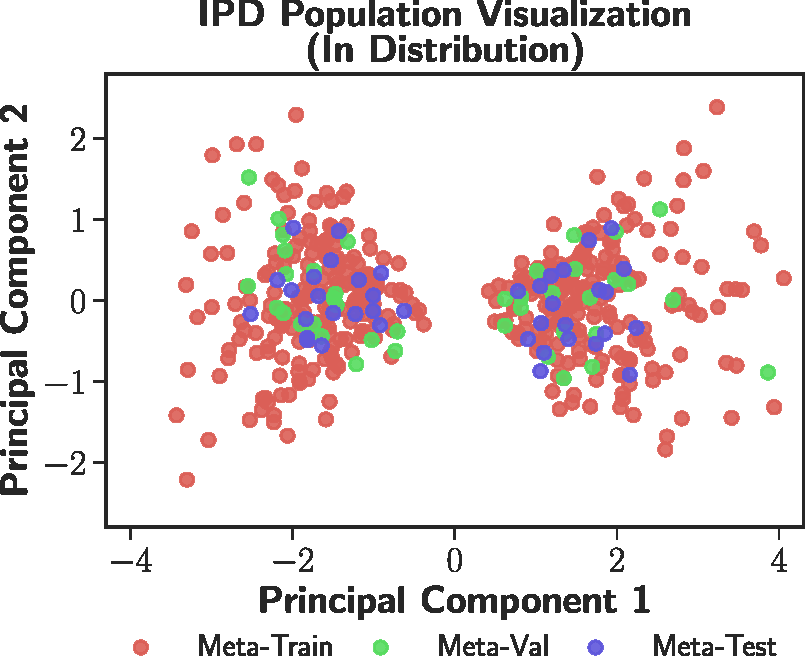
\includegraphics[height=2.9cm]{figs/pca_ipd.pdf}
        \caption{}
        \label{fig:ipd-pca}
    \end{subfigure}
    \begin{subfigure}[b]{0.45\linewidth}
        \centering
        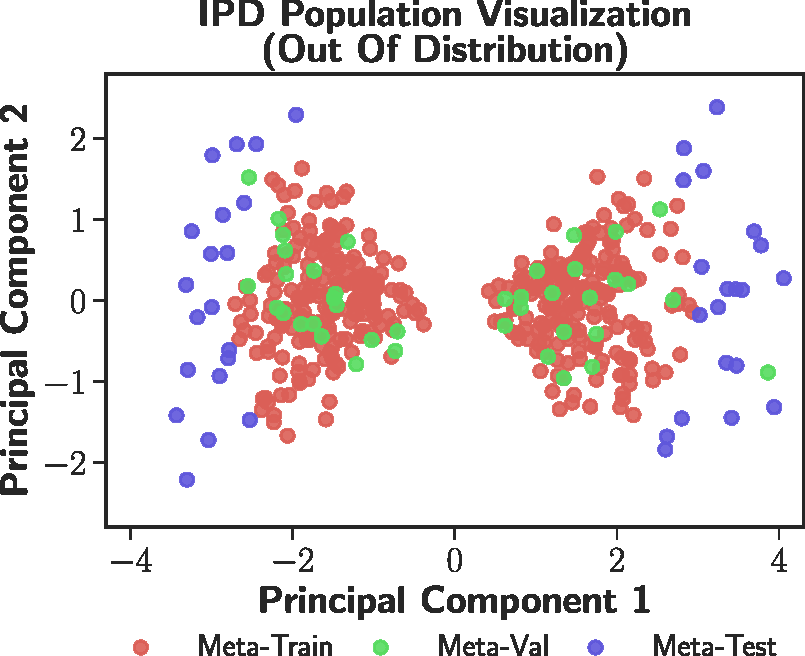
\includegraphics[height=2.9cm]{figs/pca_ipd_ood.pdf}
        \caption{}
        \label{fig:ipd-pca-ood}
    \end{subfigure}
    \vspace{-0.4cm}
    \caption{
    (\textbf{a}) and (\textbf{b}) Visualization of $j$'s initial policy for in distribution and out of distribution meta-testing, respectively, where the out of distribution split has a smaller overlap between the policies used for meta-training/validation and those used for meta-testing.}
\end{figure}
%%%%%%%%%%%%%%%%%%%%%%%%%%%%%%
\vspace{-0.8cm}

% %%%%%%%%%%%%%%%%%%%%%%%%%%%%%%%%%%%%%%%%%%%%%%%%
% \begin{figure}[t!]
% \captionsetup[subfigure]{skip=0pt}
%    \begin{subfigure}[b]{0.445\linewidth}
%         \centering
%         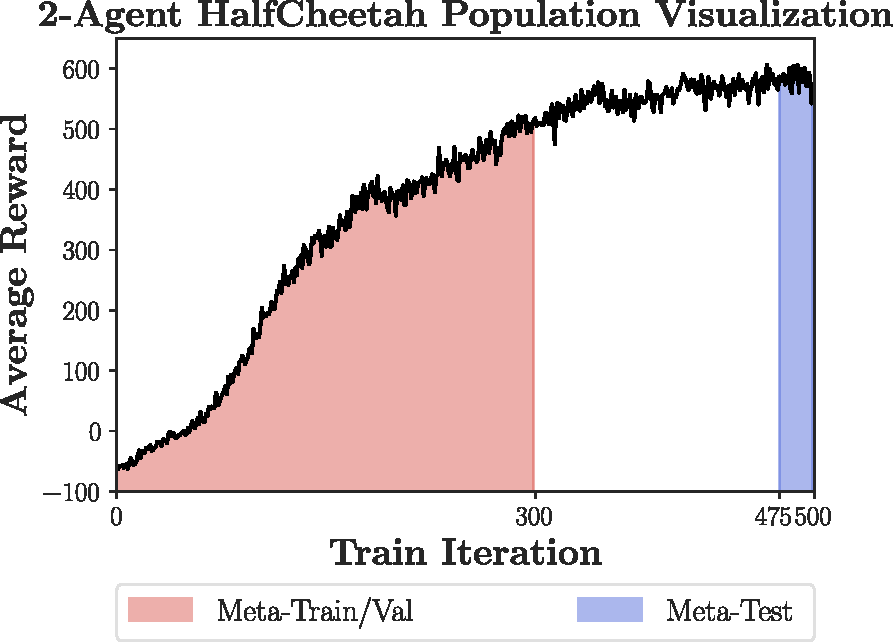
\includegraphics[height=4cm]{figs/teammate_population.pdf}
%         \caption{}
%         \label{fig:mujoco-teammate-vis}
%     \end{subfigure}
%    \begin{subfigure}[b]{0.45\linewidth}
%         \centering
%         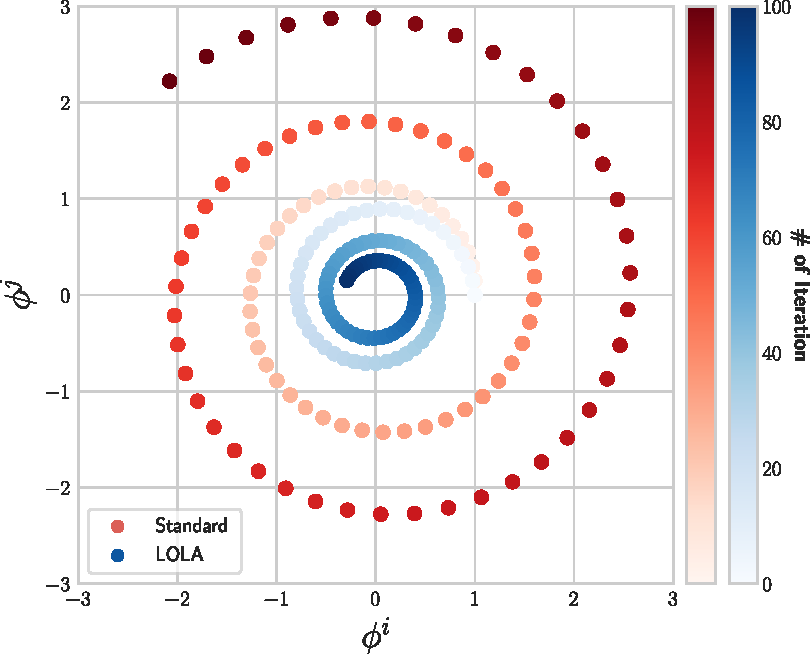
\includegraphics[height=4cm]{figs/zero_sum_exp.pdf}
%         \caption{}
%         \label{fig:zero-sum-result}
%     \end{subfigure}
%     \caption{(\textbf{a}) 
% Visualization of a teammate $j$'s initial expertise in the $2$-Agent HalfCheetah domain, where the meta-test distribution has a sufficient difference to meta-train/val. 
% (\textbf{b}) Learning paths on the zero-sum game. The standard approach with the stationary assumption diverges, resulting in worse performance for both agents. In contrast, an approach that considers the learning process of the other agents, such as LOLA~\citep{foerster17lola}, converges to the equilibrium.
%     \dXX{change legend for b}
%     }
% \end{figure}
% %%%%%%%%%%%%%%%%%%%%%%%%%%%%%%%%%%%%%%%%%%%%%%%%

\subsection{RPS}
In RPS, we follow the same meta-learning setup as in IPD, except we sample a total of $720$ initial opponent personas, including rock, paper, and scissors personas, and split them into $600$ for meta-training, $60$ for meta-validation, and $60$ for meta-testing. 
Additionally, because RPS has three possible actions, we sample a rock preference probability between $1/3$ and $1$ for building the rock persona population, where the rock probability is larger than the other two action probabilities. We follow the same procedure for constructing the paper and scissors persona population.

% \subsection{2-Agent HalfCheetah}
% We used an open source implementation for multiagent-MuJoCo benchmark.\footnote{Available at \url{https://github.com/schroederdewitt/multiagent_mujoco}}
% Agents in our experiments receive state observations that include information about all the joints.
% For the meta-learning setup, we pre-train a teammate $j$ with an LSTM policy that has varying expertise in moving to the left direction. 
% Specifically, we train the teammate up to $500$ train iterations and save a checkpoint at each iteration. 
% Intuitively, as the number of train iteration increases, the teammate gains more expertise.
% We then use the checkpoints from $50$ to $300$ iterations as the meta-train/val and from $475$ and $500$ iterations as the meta-test distribution (see~\cref{fig:mujoco-teammate-vis}). 
% We construct the distribution with the gap to ensure that the meta-testing distribution has a sufficient difference to the meta-train/val so that we can test the generalization of our approach.
% Lastly, the teammate agent $j$ updates its policy based on the policy gradient with the linear feature baseline as in IPD and RPS.

\subsection{2-Agent HalfCheetah}
\begin{wrapfigure}{r}{0.3\textwidth}
  \centering
  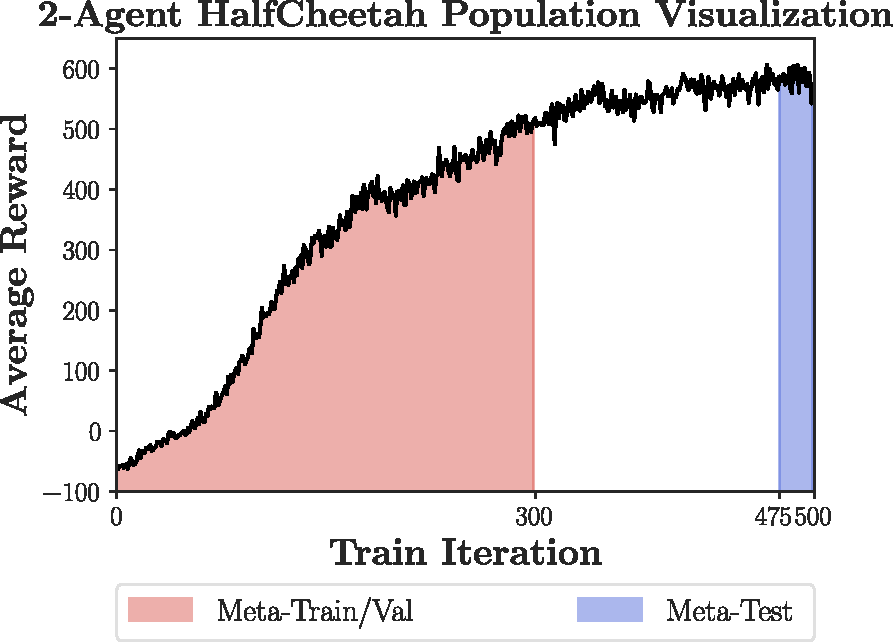
\includegraphics[width=0.75\linewidth]{figs/teammate_population.pdf}
  \caption{Visualization of a teammate $j$'s initial expertise in the $2$-Agent HalfCheetah domain, where the meta-test distribution has a sufficient difference to meta-train/val.}
  \label{fig:mujoco-teammate-vis}
\end{wrapfigure}
We used an open source implementation for multiagent-MuJoCo benchmark: \url{https://github.com/schroederdewitt/multiagent_mujoco}.
Agents in our experiments receive state observations that include information about all the joints.
For the meta-learning setup, we pre-train a teammate $j$ with an LSTM policy that has varying expertise in moving to the left direction. 
Specifically, we train the teammate up to $500$ train iterations and save a checkpoint at each iteration. 
Intuitively, as the number of train iteration increases, the teammate gains more expertise.
We then use the checkpoints from $0$ to $300$ iterations as the meta-train/val (randomly split them into $275$ for meta-training and $25$ for meta-validation) and from $475$ and $500$ iterations as the meta-test distribution (see~\cref{fig:mujoco-teammate-vis}). 
We construct the distribution with the gap to ensure that the meta-testing distribution has a sufficient difference to the meta-train/val so that we can test the generalization of our approach.
As in IPD and RPS, the teammate $j$ updates its policy based on the policy gradient with the linear feature baseline.

% \section{Importance of Peer Learning}\label{sec:importance-peer-learning}
% \begin{wrapfigure}{r}{0.34\textwidth}
%   \centering
%   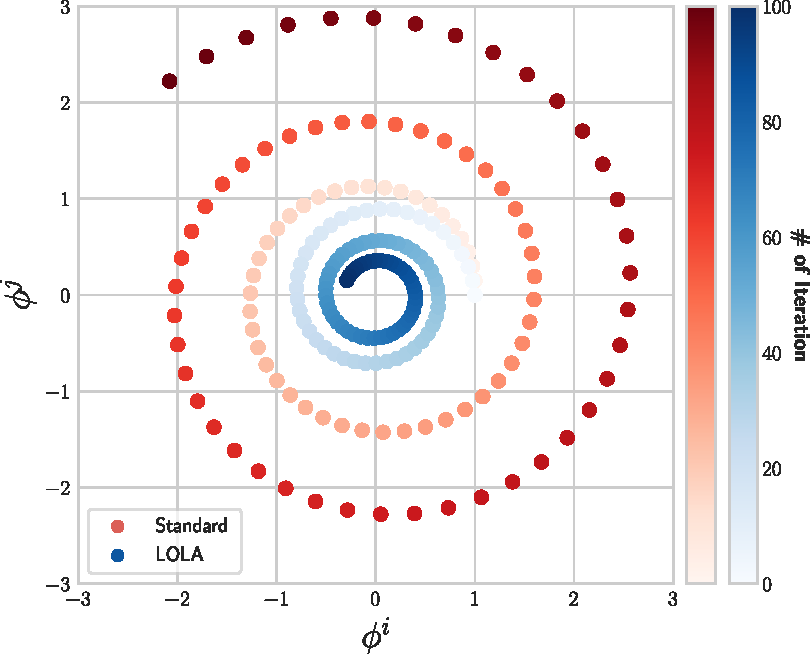
\includegraphics[width=0.84\linewidth]{figs/zero_sum_exp.pdf}
%   \caption{Learning paths on the zero-sum game between the standard and LOLA method.}
%   % The standard approach with the stationary assumption diverges, resulting in worse performance for both agents.
%   % In contrast, an approach that considers the learning process of the other agents, such as LOLA~\citep{foerster17lola}, converges to the equilibrium.  
%   \label{fig:zero-sum-result}
% \end{wrapfigure}

% \begin{example}\label{remark:divergence-of-learning-objective}
% Failure to consider the learning process of the other agents can result in divergence of learning objectives.
% \end{example}
% \noindent
% For example, consider a stateless zero-sum game playing between two agents.
% Agents $i$ and $j$ maximize simple value functions $V^{i}_{\bm{\phi}}\!=\!\phi^{i}\phi^{j}$ and $V^{j}_{\bm{\phi}}\!=\!-\phi^{i}\phi^{j}$ respectively, where $\phi^{i},\phi^{j}\!\in\!\mathbb{R}$.
% In this game, there exists a unique Nash equilibrium at the origin (i.e., $\{\phi^{i},\phi^{j}\}\!=\!\{0,0\}$). 
% We compare: 1) the standard approach that optimizes the value function in~\cref{eqn:value-function} with the stationary assumption and 2) an approach that considers the learning process of others, such as the LOLA method.
% As~\cref{fig:zero-sum-result} shows, the standard approach diverges further from the equilibrium, resulting in worse results for both agents.
% The cause of the failure in this example is due to the stationary assumption that each agent assumes its opponent has the same behavior in the future~\citep{letcher2018stable}.
% In contrast, by considering the opponent's learning process, the LOLA approach converges to the equilibrium. 
% As such, it is important to consider others' learning as highlighted by this example.\dXX{remove?}

\clearpage
\section{Analysis on Joint Policy Dynamics}\label{sec:analysis-details}
\subsection{IPD}
%%%%%%%%%%%%%%%%%%%%%%%%%%%%%%%%%%%%%%%%%%%%%%%%
\begin{figure}[H]
    \centering
    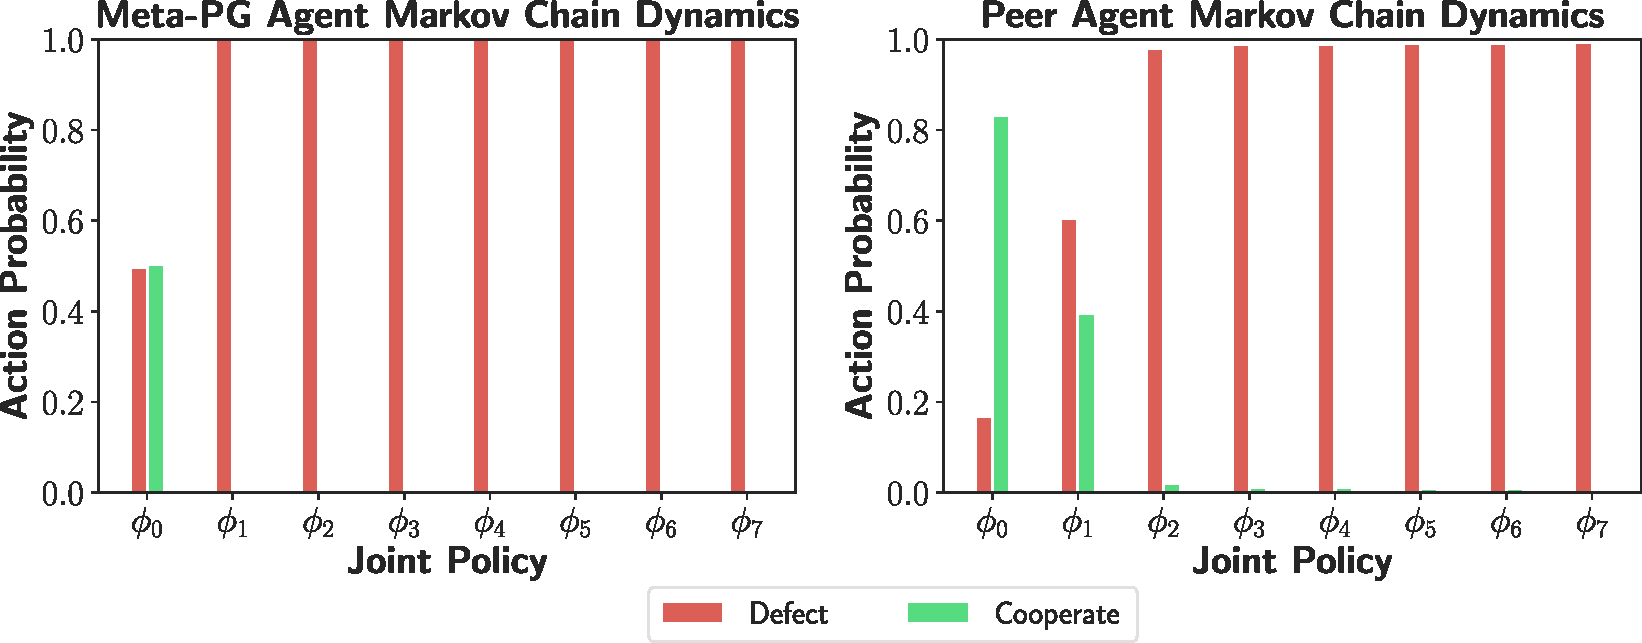
\includegraphics[width=0.59\linewidth]{figs/ipd_meta_pg_analysis.pdf}
    \caption{Action probability dynamics with Meta-PG in IPD with a cooperating persona peer}
    \label{fig:ipd-meta-pg-analysis}
\end{figure}
\begin{figure}[H]
    \centering
    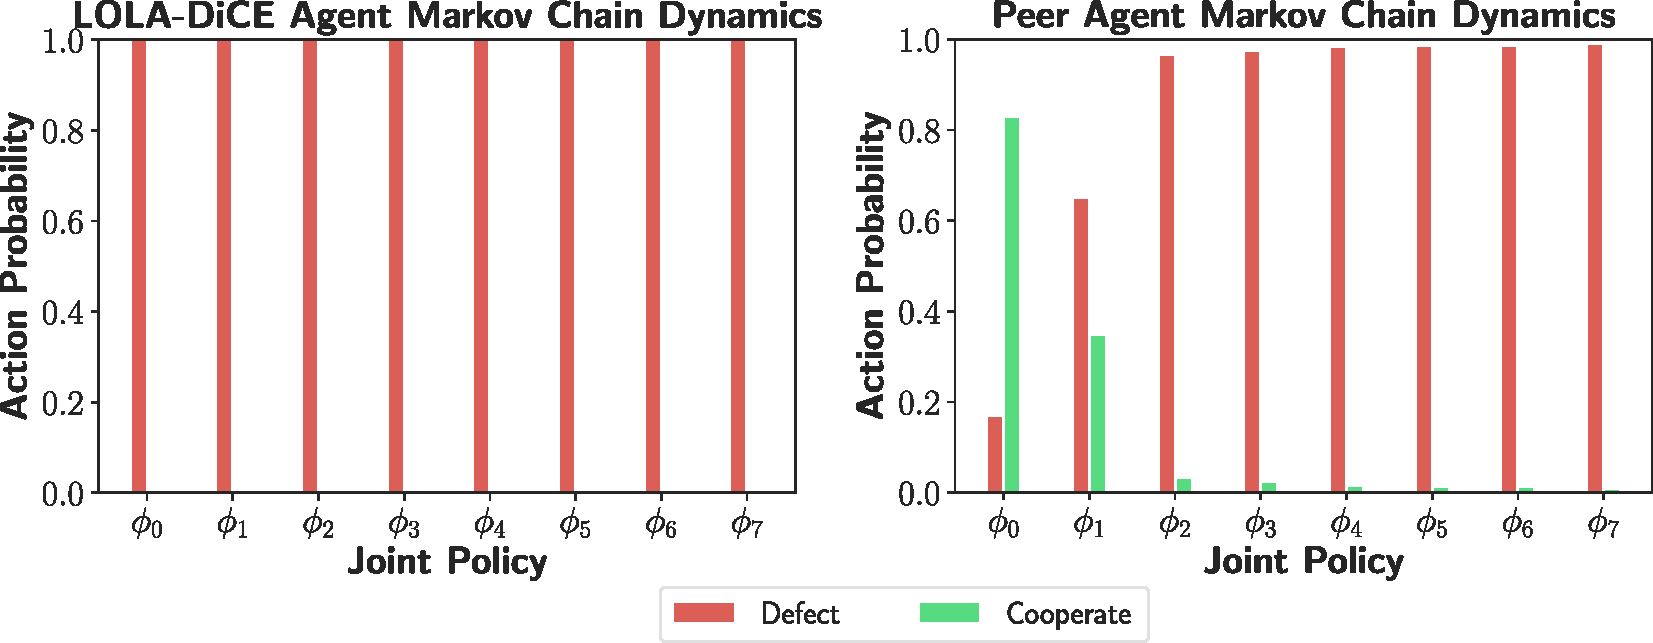
\includegraphics[width=0.59\linewidth]{figs/ipd_dice_analysis.pdf}
    \caption{Action probability dynamics with LOLA-DiCE in IPD with a cooperating persona peer}
    \label{fig:ipd-dice-analysis}
\end{figure}
\begin{figure}[H]
    \centering
    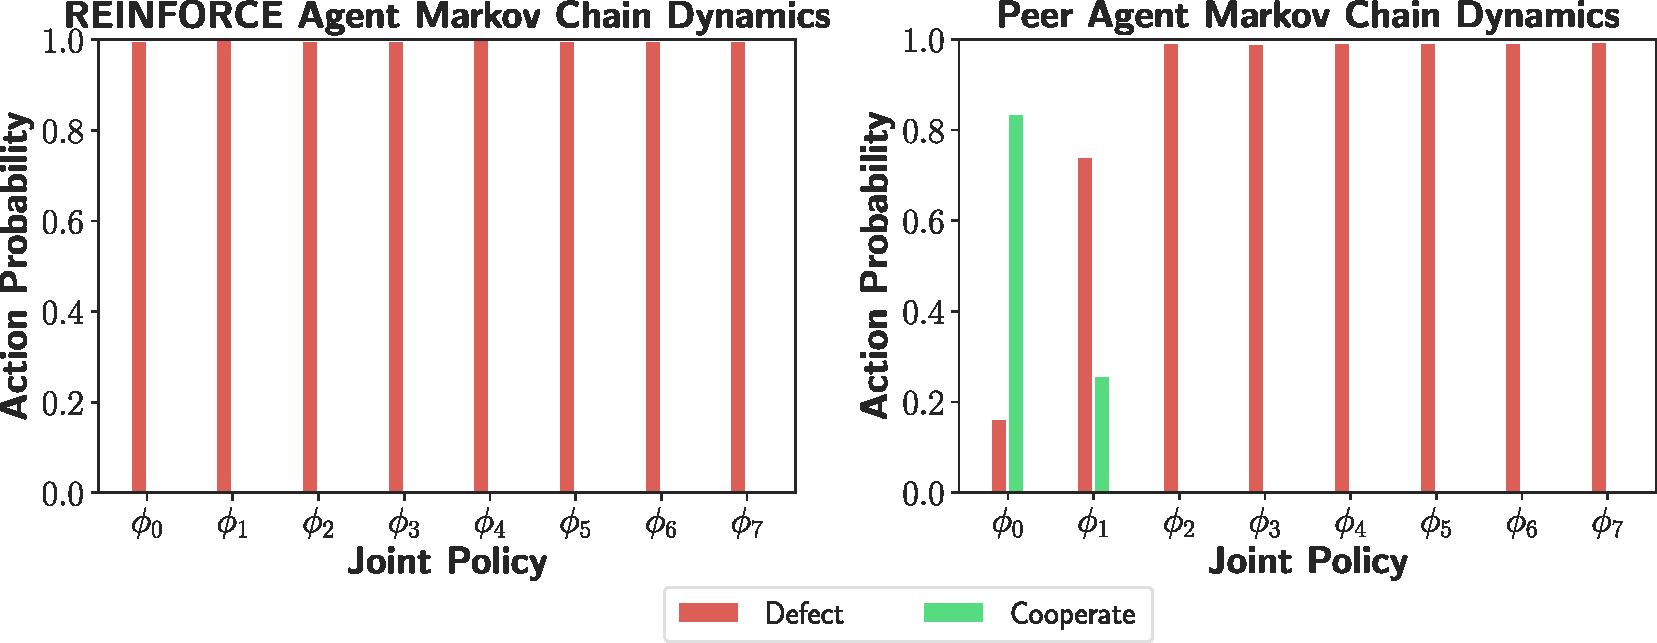
\includegraphics[width=0.59\linewidth]{figs/ipd_reinforce_analysis.pdf}
    \caption{Action probability dynamics with REINFORCE in IPD with a cooperating persona peer}
    \label{fig:ipd-reinforce-analysis}
\end{figure}
\begin{figure}[H]
    \centering
    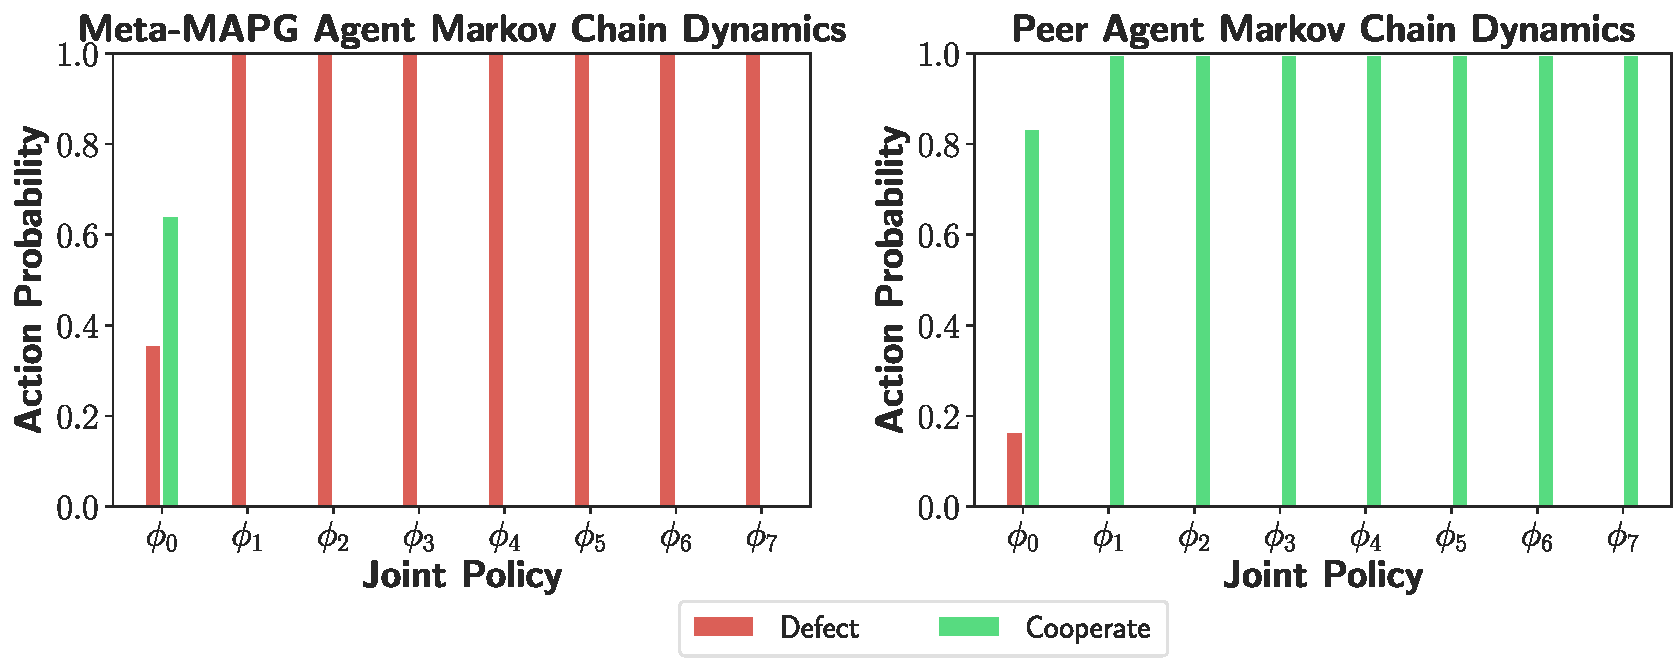
\includegraphics[width=0.59\linewidth]{figs/ipd_meta_mapg_analysis.pdf}
    \caption{Action probability dynamics with Meta-MAPG in IPD with a cooperating persona peer}
    \label{fig:ipd-meta-mapg-analysis}
\end{figure}
%%%%%%%%%%%%%%%%%%%%%%%%%%%%%%%%%%%%%%%%%%%%%%%%

\subsection{RPS}
%%%%%%%%%%%%%%%%%%%%%%%%%%%%%%%%%%%%%%%%%%%%%%%%
\begin{figure}[H]
    \centering
    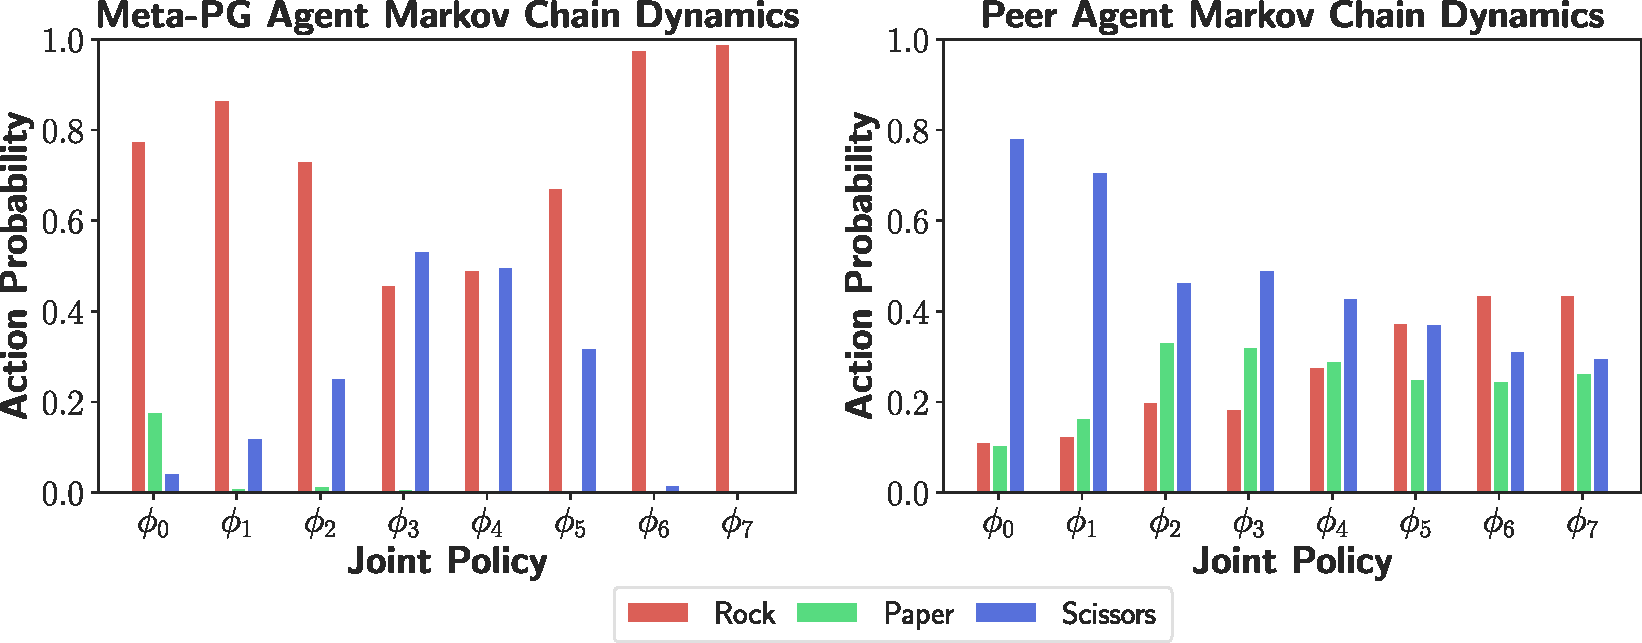
\includegraphics[width=0.59\linewidth]{figs/rps_meta_pg_analysis.pdf}
    \caption{Action Probability Dynamics with Meta-PG in RPS with a scissors persona opponent}
    \label{fig:rps-meta-pg-analysis}
\end{figure}
\begin{figure}[H]
    \centering
    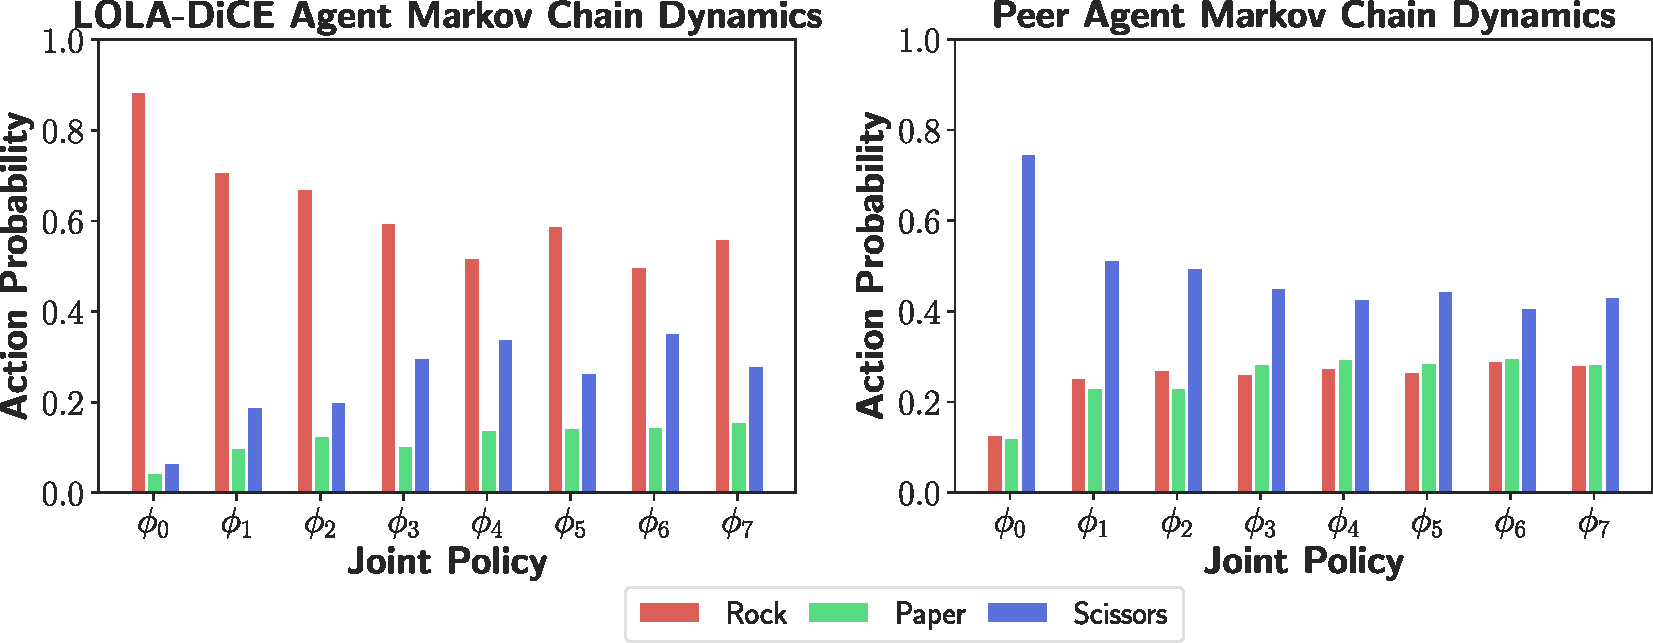
\includegraphics[width=0.59\linewidth]{figs/rps_dice_analysis.pdf}
    \caption{Action Probability Dynamics with LOLA-DiCE in RPS with a scissors persona opponent}
    \label{fig:rps-dice-analysis}
\end{figure}
\begin{figure}[H]
    \centering
    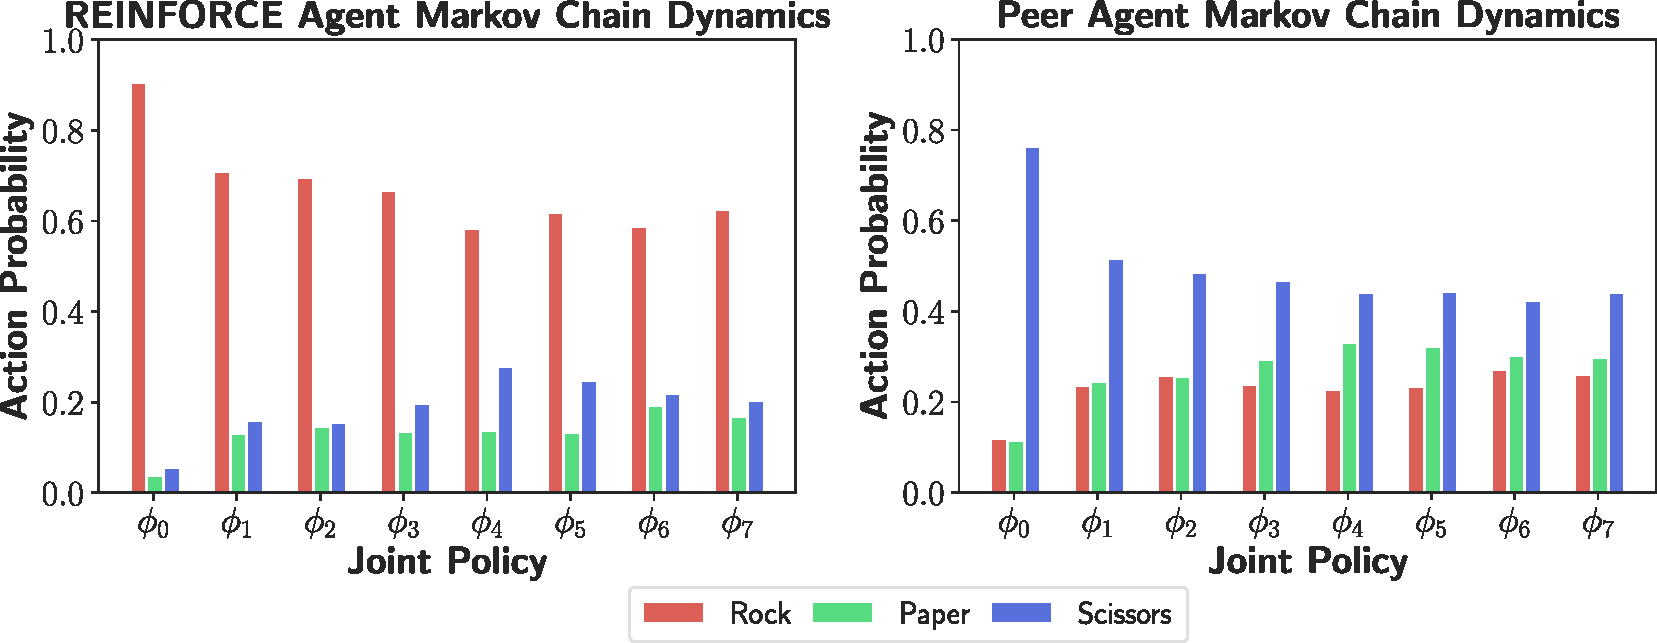
\includegraphics[width=0.59\linewidth]{figs/rps_reinforce_analysis.pdf}
    \caption{Action Probability Dynamics with REINFORCE in RPS with a scissors persona opponent}
    \label{fig:rps-reinforce-analysis}
\end{figure}
\begin{figure}[H]
    \centering
    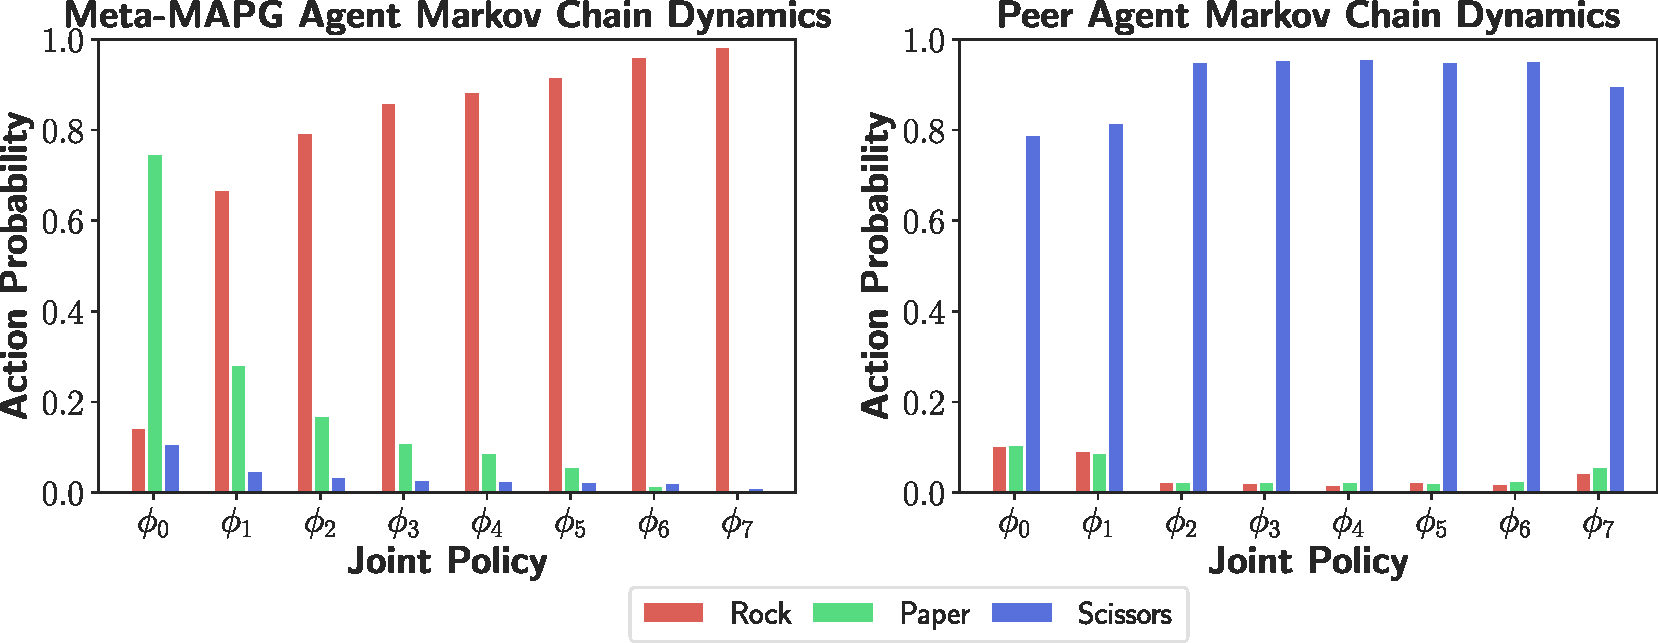
\includegraphics[width=0.59\linewidth]{figs/rps_meta_mapg_analysis.pdf}
    \caption{Action Probability Dynamics with Meta-MAPG in RPS with a scissors persona opponent}
    \label{fig:rps-meta-mapg-analysis}
\end{figure}
%%%%%%%%%%%%%%%%%%%%%%%%%%%%%%%%%%%%%%%%%%%%%%%%

\section{Hyperparameter Details}\label{sec:hyperparameter-details}
We report our hyperparameter values that we used for each of the methods in our experiments:
\subsection{Meta-MAPG and Meta-PG}
\begin{table}[H]
\centering
\begin{tabular}{l|l}
Hyperparameter & Value \\ \hline
Trajectory batch size $K$ & 4, 8, 16, 32, 64 \\
Number of parallel threads & 5 \\
Actor learning rate (inner) & 1.0, 0.1 \\
Actor learning rate (outer) & 1e-4 \\
Critic learning rate (outer) & 1.5e-4 \\
Episode horizon $H$ & 150 \\
Max chain length $L$ & 7 \\
GAE $\lambda$ & 0.95 \\
Discount factor $\gamma$ & 0.96 \\
\end{tabular}
\caption{IPD}
\end{table}

\begin{table}[H]
\centering
\begin{tabular}{l|l}
Hyperparameter & Value \\ \hline
Trajectory batch size $K$ & 64 \\
Number of parallel threads & 5 \\
Actor learning rate (inner) & 0.01 \\
Actor learning rate (outer) & 1e-5 \\
Critic learning rate (outer) & 1.5e-5 \\
Episode horizon $H$ & 150 \\
Max chain length $L$ & 7 \\
GAE $\lambda$ & 0.95 \\
Discount factor $\gamma$ & 0.90 \\
\end{tabular}
\caption{RPS}
\end{table}

\begin{table}[H]
\centering
\begin{tabular}{l|l}
Hyperparameter & Value \\ \hline
Trajectory batch size $K$ & 64 \\
Number of parallel threads & 5 \\
Actor learning rate (inner) & 0.005 \\
Actor learning rate (outer) & 5e-5 \\
Critic learning rate (outer) & 5.5e-5 \\
Episode horizon $H$ & 200 \\
Max chain length $L$ & 2 \\
GAE $\lambda$ & 0.95 \\
Discount factor $\gamma$ & 0.95 \\
\end{tabular}
\caption{$2$-Agent HalfCheetah}
\end{table}

\subsection{LOLA-DiCE}
\begin{table}[H]
\centering
\begin{tabular}{l|l}
Hyperparameter & Value \\ \hline
Trajectory batch size $K$ & 4, 8, 16, 32, 64 \\
Actor learning rate & 1.0, 0.1 \\
Critic learning rate & 1.5e-3 \\
Episode horizon $H$ & 150 \\
Max chain length $L$ & 7 \\
Number of Look-Ahead & 1, 3, 5 \\
Discount factor $\gamma$ & 0.96 \\
\end{tabular}
\caption{IPD}
\end{table}

\begin{table}[H]
\centering
\begin{tabular}{l|l}
Hyperparameter & Value \\ \hline
Trajectory batch size $K$ & 64 \\
Actor learning rate & 0.01 \\
Critic learning rate & 1.5e-5 \\
Episode horizon $H$ & 150 \\
Max chain length $L$ & 7 \\
Number of Look-Ahead & 1 \\
Discount factor $\gamma$ & 0.90 \\
\end{tabular}
\caption{RPS}
\end{table}

\begin{table}[H]
\centering
\begin{tabular}{l|l}
Hyperparameter & Value \\ \hline
Trajectory batch size $K$ & 64 \\
Actor learning rate & 0.005 \\
Critic learning rate & 5.5e-5 \\
Episode horizon $H$ & 200 \\
Max chain length $L$ & 2 \\
Number of Look-Ahead & 1 \\
Discount factor $\gamma$ & 0.95 \\
\end{tabular}
\caption{$2$-Agent HalfCheetah}
\end{table}

\subsection{REINFORCE}
\begin{table}[H]
\centering
\begin{tabular}{l|l}
Hyperparameter & Value \\ \hline
Trajectory batch size $K$ & 4, 8, 16, 32, 64 \\
Actor learning rate & 1.0, 0.1 \\
Episode horizon $H$ & 150 \\
Max chain length $L$ & 7 \\
Discount factor $\gamma$ & 0.96 \\
\end{tabular}
\caption{IPD}
\end{table}

\begin{table}[H]
\centering
\begin{tabular}{l|l}
Hyperparameter & Value \\ \hline
Trajectory batch size $K$ & 64 \\
Actor learning rate & 0.01 \\
Episode horizon $H$ & 150 \\
Max chain length $L$ & 7 \\
Discount factor $\gamma$ & 0.90 \\
\end{tabular}
\caption{RPS}
\end{table}

\begin{table}[H]
\centering
\begin{tabular}{l|l}
Hyperparameter & Value \\ \hline
Trajectory batch size $K$ & 64 \\
Actor learning rate & 0.005 \\
Episode horizon $H$ & 200 \\
Max chain length $L$ & 2 \\
Discount factor $\gamma$ & 0.95 \\
\end{tabular}
\caption{$2$-Agent HalfCheetah}
\end{table}